%! TEX root = ../../master.tex
\lecture[Further intuition why IP is hard. Big-$\mathcal{O}$ notation]{Th 21 Apr 2022}{Introduction II}

\begin{theorem}
    $\IP$ can approximate any objective function infinitely good.\label{thm:ip-piecewise-model}
\end{theorem}

\begin{proof}
    First, consider a \vocab[objective function!piecewise linear]{piecewise linear} objective function $f$
    with (not necessarily equidistant) breakpoints $a_1,\dots,a_k$.
    \\
    \begin{minipage}{\textwidth}
        \centering
        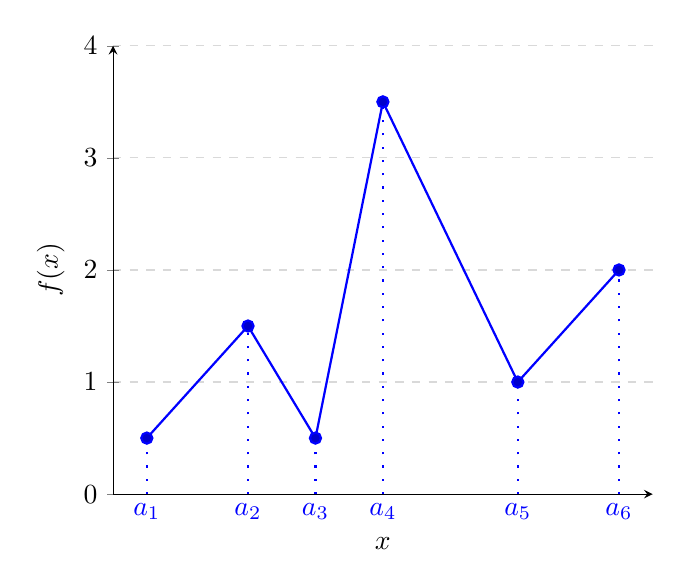
\begin{tikzpicture}
            \begin{axis}[
                    axis x line=bottom,
                    axis y line=left,
                    grid = major,
                    grid style={dashed, gray!30},
                    % width = 16cm,
                    % height = 8cm,
                    xmin = 0,
                    xmax = 8,
                    ymin = 0,
                    ymax = 4,
                    xlabel = $x$,
                    ylabel = $f(x)$,
                    xlabel shift = 10,
                    xtick = \empty
                ]
                % \addplot[domain=1:8, blue, thick, samples=100]{x < 2 ? 0.5*x : (x < 4 ? x - 1 : (x < 5 ? 11 - 2 *x : 1.5 *x-9))};
                \addplot+[blue,thick] coordinates {
                        (0.5, 0.5)
                        (2,1.5)
                        (3, 0.5)
                        (4, 3.5)
                        (6, 1)
                        (7.5, 2)
                    };
                \addplot[ycomb,
                    blue,thick,loosely dotted,
                    symbolic x coords={a,b,c,d,e,f}
                ] coordinates {
                        (0.5, 0.5)
                        (2,1.5)
                        (3, 0.5)
                        (4, 3.5)
                        (6, 1)
                        (7.5, 2)
                    };
                \addplot[blue,nodes near coords,
                    nodes near coords align=below,
                    only marks,
                    point meta=explicit symbolic]
                coordinates {
                        (0.5, 0) [$a_1$]
                        (2,0) [$a_2$]
                        (3, 0) [$a_3$]
                        (4, 0) [$a_4$]
                        (6, 0) [$a_5$]
                        (7.5, 0) [$a_6$]
                    };
            \end{axis}
        \end{tikzpicture}
        \captionof{figure}{A piecewise linear function}
    \end{minipage}
    \\
    Defining the intervals $I_i \coloneqq [a_i,a_{i+1}]$ for each segment of $f$, we can introduce binary variables $y_i$ such that
    \begin{align*}
        y_i = \begin{cases}
                  1, & \text{if } x \in I_i, \\
                  0, & \text{otherwise}
              \end{cases}
    \end{align*}
    Note that for $x \in I_i$, $x$ is a convex combination of $a_i,a_{i+1}$.
    Therefore, we can express $x$ as a linear combination of all breakpoints $a_i$, with the additional constraint that
    all except 2 scalars must be $0$. By linearity, this also holds for $f(x)$. Translating into $\IP$:
    \begin{mini*}{\lambda}{\sum_i \lambda_i f(a_i)}{}{}
        \addConstraint{\lambda_1}{\leq y_1}
        \addConstraint{\lambda_k}{\leq y_{k-1}}
        \addConstraint{\lambda_{i}}{\leq y_{i-1} + y_i, \quad}{i = 2,\dots,k-1}
        \addConstraint{\sum_i y_i}{=1}
    \end{mini*}
    One can show this already suffices to model any cost function: For suitable
    choices of breakpoints we can approximate any function by piecewise linear functions.
    Details can be found in \cite[Ch. 14]{network-flows} or \cite[Ch. 1]{int-comb-optimization}.
\end{proof}

\begin{conclusion}
    Summarizing, following facts that hold for $\IP$, but not $\LP$, deliver an intuition why $\IP$ should be hard:
    \begin{enumerate}
        \item Consider a polyhedron $P = \{x \in \realnum^n \mid Ax=b\}$ and its integer hull $Q$.
              Even though $P$ can be "smooth" (e.g. cube), its integer hull can look more like a "disco ball" with many facets.
        \item In real life, many problems can be modeled with decision variables. $\IP$ can handle this, see \autoref{thm:ip-logical-decomposition}.
        \item Additionally, $\IP$ also can handle non-convex problems, see \autoref{thm:ip-model-union} and \autoref{thm:ip-piecewise-model}.
    \end{enumerate}
\end{conclusion}

\subsection{Representation of $\IP$s}
For a given $\IP$, a set $Q$ of feasible points can be formulated by many polyhedra $P$.
\begin{example}
    Consider
    \begin{align*}
        Q \coloneqq & \ \{0000,1000,0100,0010,0110,0101,0011\} \subseteq \integers^4.
    \end{align*}
    Then we can give following representations $P_i$ such that $P_i$ is an integer hull of $Q$:
    \begin{alignat*}{2}
        P_1 =\  & \{x \in \realnum^4  \mid \  & 93 x_1 + 49x_2 + 37x_3+29x_4 & \leq 111\} \\
        P_2 =\  & \{x \in \realnum^4  \mid    & 2 x_1 + x_2 + x_3+ x_4       & \leq 2\}   \\
        P_3 =\  & \{x \in \realnum^4  \mid    & 2 x_1 + x_2 + x_3+ x_4       & \leq 2,    \\
                &                             & x_1 + x_2                    & \leq 1,    \\
                &                             & x_1 + x_3                    & \leq 1,    \\
                &                             & x_1 + x_4                    & \leq 1\}
    \end{alignat*}
    One can show that $P_3 \subsetneq P_2 \subsetneq P_1$.
\end{example}
\begin{example}
    A real-life example is the problem of placing facilities.
    Given $n$ stores and $m$ warehouses, decide which warehouse should be build at all, and which should deliver which store (for some cost function).
    Let $y_i \in \bool$ denote if warehouse $i$ should be opened, and $x_{ij}$ if warehouse $i$ should serve store $j$.
    Then
    \begin{alignat*}{2}
        P_1 \coloneqq \  & \{x \mid \  & \forall i: \sum_j x_{ij} & \leq my_i \}, \\
        P_2 \coloneqq \  & \{x \mid \  & \forall i,j: x_{ij}      & \leq y_i\}    \\
    \end{alignat*}
    both represent the condition to only serve stores from warehouses that are opened.
    Notice that $P_2 \subsetneq P_1$ is tighter, but has $n \cdot m$ instead of $n$ constraints.
\end{example}

\subsection{Complexity}
In order to define hardness, it is useful to define complexity first.
We can use \vocab[big-O]{big-$\mathcal{O}$} for this. During the rest of the lecture,
we had a recap on this. For details, refer to canonical sources.
